\documentclass[10 pt,usenames,dvipsnames, oneside]{article}
\usepackage{../../../modelo-ensino-medio}



\begin{document}

\begin{center}
  \begin{minipage}[l]{3cm}

\includegraphics[width=2cm]{logo}    
\end{minipage}\hfill
\begin{minipage}[r]{.8\textwidth}
 {\Large \scshape Atividade: Construindo o próprio pêndulo}  
\end{minipage}
\end{center}
\vspace{.2cm}

\ifdefined\prof
%Habilidades da BNCC
% \begin{objetivos}
% \item 
% \end{objetivos}

%Caixa do Para o Professor
\begin{goals}
%Objetivos específicos
\begin{enumerate}
\item Apresentar os fenômenos periódicos por uma perspectiva
empírica
\item Construir gráfico de fenômeno que pode ser modelado por
função periódica
\end{enumerate}

\tcblower

%Orientações e sugestões
Ao término dessa atividade, é importante comparar
os gráficos obtidos com aqueles construídos na atividade
anterior. Como o movimento a ser modelado nas duas
atividades é essencialmente o mesmo, o gráfico construído
nesta segunda atividade, de forma experimental e com mais
precisão contribuirá para que o aluno reflita sobre possíveis
imperfeições existentes no formato dos gráficos obtidos na
atividade anterior.

Uma outra maneira de se construir um pêndulo simples, mas
com borracha, tubo de caneta, linha de costura e fita adesiva
pode ser visto na atividade 5 de: \url{http://www.aprendizagemconectada.mt.gov.br/documents/14
069491/14094177/Semana+04-08+de+maio/cb1df5e3-7082-
b9a1-be1f-714c5f25265d}
\end{goals}

\bigskip
\begin{center}
{\large \scshape Atividade}
\end{center}
\fi

\textit{(Adaptado de Costa (2017))}
\label{trig-ativ2}

Com madeira, um prego, barbante e uma bolinha de gude, construir um pêndulo como o da figura. 

\begin{figure}[H]
\centering

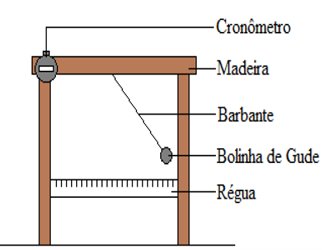
\includegraphics[height=.225\textheight]{trigonometricas5}
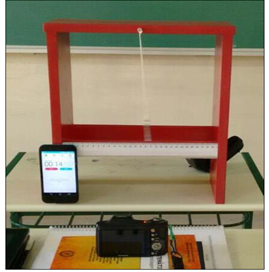
\includegraphics[height=.225\textheight]{trigonometricas6}

\caption{Fonte: Costa (2017)}
\end{figure}

Será necessário o uso de dois celulares ou um celular e uma câmera. Um dos celulares irá cronometrar o tempo durante a oscilação do pêndulo e o outro, deverá tirar sucessivas fotografias do movimento do pêndulo e do primeiro celular. Uma régua deve ser utilizada também para medir o deslocamento horizontal da projeção do pêndulo, como na figura acima. Posicione o pêndulo exatamente sobre o zero da régua e solte-o no momento em que cronômetro for ligado e as fotos começarem a ser tiradas. Fotografar o movimento ao longo de 4 oscilações completas do pêndulo.

\begin{enumerate}
\item Analise as fotografias e forme pares ordenados $(x,y)$ onde $x$ representa o tempo e $y$, a medida na régua na qual estará a projeção horizontal do pêndulo.

\item Plote os pontos no GeoGebra. Que comportamento você consegue perceber no caminho que os pontos vão percorrendo?
\item Compare o esboço que você obteve aqui com o da atividade anterior. Que conclusões você consegue tirar?
\end{enumerate}

\ifdefined\prof
\begin{solucao}

\begin{enumerate}
\item ---
\item Movimento de “sobe e desce”{} e de repetição do mesmo
com o passar do tempo (movimento periódico)
\item São similares, com repetição de um padrão, mas neste
último gráfico, o formato arredondado ficará mais evidente,
fazendo com que o aluno reflita sobre possíveis imperfeições
nos desenhos da atividade anterior
\end{enumerate}
\end{solucao}
\fi

\end{document}